% !TEX program = xelatex
\makeatletter\let\@expl@@@mark@update@singlecol@structures@@\relax\makeatother
\documentclass[10pt,a4paper]{article}

% -------------------- កញ្ចប់ពុម្ពអក្សរ និងភាសា --------------------
\usepackage{fontspec}
\usepackage{amsmath,amssymb}
\usepackage{unicode-math}
\usepackage{pifont}

% -------------------- ការកំណត់ទំព័រ (៣ ទំព័រ A4 ស-ខ្មៅ តម្រៀបបញ្ឈរច្បាស់លាស់) --------------------
\usepackage[
  a4paper,
  left=1.10cm,
  right=1.10cm,
  top=0.95cm,
  bottom=1.10cm,
  footskip=0.52cm
]{geometry}

\usepackage{fancyhdr}
\usepackage{lastpage}
\usepackage{array}
\usepackage{colortbl}
\usepackage[table]{xcolor}
\usepackage{enumitem}
\usepackage{tikz}
\usetikzlibrary{calc,angles,quotes,arrows.meta,decorations.pathreplacing}
\usepackage[most]{tcolorbox}

% -------------------- ពុម្ពអក្សរផ្លូវការ (Cross-Platform \NGSFindFonts) --------------------
\providecommand{\NGSFindFonts}{%
  \IfFileExists{C:/Windows/Fonts/cambria.ttc}{%
    \def\NGSSysPath{C:/Windows/Fonts/}%
    \def\NGSUserPath{C:/Users/KIT/AppData/Local/Microsoft/Windows/Fonts/}%
  }{%
    \IfFileExists{./fonts/KhmerOSsiemreap.ttf}{\def\NGSSysPath{./fonts/}\def\NGSUserPath{./fonts/}}{%
    \IfFileExists{../fonts/KhmerOSsiemreap.ttf}{\def\NGSSysPath{../fonts/}\def\NGSUserPath{../fonts/}}{%
    \IfFileExists{../../fonts/KhmerOSsiemreap.ttf}{\def\NGSSysPath{../../fonts/}\def\NGSUserPath{../../fonts/}}{%
    \IfFileExists{../../../fonts/KhmerOSsiemreap.ttf}{\def\NGSSysPath{../../../fonts/}\def\NGSUserPath{../../../fonts/}}{%
    \IfFileExists{../../../../fonts/KhmerOSsiemreap.ttf}{\def\NGSSysPath{../../../../fonts/}\def\NGSUserPath{../../../../fonts/}}{%
    \IfFileExists{../../../../../fonts/KhmerOSsiemreap.ttf}{\def\NGSSysPath{../../../../../fonts/}\def\NGSUserPath{../../../../../fonts/}}{%
    \IfFileExists{../../../../../../fonts/KhmerOSsiemreap.ttf}{\def\NGSSysPath{../../../../../../fonts/}\def\NGSUserPath{../../../../../../fonts/}}{%
      \def\NGSSysPath{../../../../../../../fonts/}\def\NGSUserPath{../../../../../../../fonts/}%
    }}}}}}}%
  }%
}
\NGSFindFonts

\setmathfont[Path={\NGSSysPath}, FontIndex=1, Scale=1.02]{cambria.ttc}
\defaultfontfeatures{Ligatures=TeX}

\setmainfont[
  Path={\NGSUserPath}, Extension=.ttf, Script=Khmer,
  BoldFont={KhmerOSsiemreap}, BoldFeatures={FakeBold=1.8},
  ItalicFont={KhmerOSsiemreap}, ItalicFeatures={FakeSlant=0.22},
  BoldItalicFont={KhmerOSsiemreap}, BoldItalicFeatures={FakeBold=1.8, FakeSlant=0.22}
]{KhmerOSsiemreap}

\newfontfamily\muol[Path={\NGSUserPath}, Extension=.ttf, Script=Khmer]{KhmerOSmuollight}
\newfontfamily\LatinFont[Path={\NGSSysPath}, Extension=.ttf, BoldFont={timesbd}, ItalicFont={timesi}, BoldItalicFont={timesbi}]{times}

\XeTeXlinebreaklocale "km"
\XeTeXlinebreakskip = 0pt plus 1pt minus 0.1pt

\definecolor{panelgray}{HTML}{F2F2F2}
\definecolor{headband}{HTML}{E4E4E4}

\newlist{wlist}{itemize}{1}
\setlist[wlist]{label=\textbullet, leftmargin=1.35em, itemsep=2.5pt, topsep=2pt, parsep=0pt, partopsep=0pt}

\newlist{subwlist}{itemize}{1}
\setlist[subwlist]{label=\textendash, leftmargin=1.25em, itemsep=2.5pt, topsep=2pt, parsep=0pt, partopsep=0pt}

\newcommand{\en}[1]{{\LatinFont #1}}
\newcommand{\enbf}[1]{{\LatinFont\textbf{#1}}}
\newcommand{\unit}[1]{\,\text{\en{#1}}}
\newcommand{\cnum}[1]{{\fontsize{10pt}{11pt}\selectfont\ding{\numexpr181+#1\relax}}\hspace{0.15em}}
\newcommand{\blank}[1]{\underline{\hspace{#1}}}
\newcommand{\chkbox}{\tikz[baseline=-0.3ex]\draw[black,line width=0.8pt] (0,0) rectangle (0.33,0.33);}
\newcommand{\numbox}{\tikz[baseline=-0.35ex]\draw[black,line width=0.9pt] (0,0) rectangle (0.45,0.45);}

\newcommand{\secbox}[2]{%
  \vspace{6pt}%
  \noindent\begin{tcolorbox}[
    enhanced, sharp corners, boxrule=0.9pt, colframe=black, colback=headband,
    left=7pt, right=7pt, top=4pt, bottom=4pt, boxsep=1pt
  ]
    {\muol\fontsize{9.8pt}{14pt}\selectfont #1}\hfill{\fontsize{9.0pt}{12.5pt}\selectfont\textbf{#2}}
  \end{tcolorbox}%
  \vspace{4pt}%
}

\newcolumntype{L}[1]{>{\raggedright\arraybackslash}p{#1}}
\newcolumntype{C}[1]{>{\centering\arraybackslash}p{#1}}

\pagestyle{fancy}
\fancyhf{}
\renewcommand{\headrulewidth}{0pt}
\renewcommand{\footrulewidth}{0.4pt}
\fancyfoot[L]{\fontsize{8.8pt}{11.5pt}\selectfont អនុវិទ្យាល័យព្រះក្រសាំង \en{|} គណិតវិទ្យា ថ្នាក់ទី៧ \en{---} មេរៀនទី២ (១.១ គ. ភាពចែកដាច់នឹង 4 និង 8) \en{|} គ្រូ៖ ហុក ប៊ុនថែន}
\fancyfoot[R]{\fontsize{8.8pt}{11.5pt}\selectfont ទំព័រ \en{\thepage\ / \pageref{LastPage}}}

\setlength{\parindent}{0pt}
\setlength{\parskip}{0pt}
\setlength{\tabcolsep}{4.5pt}

\begin{document}
\fontsize{9.7pt}{14.6pt}\selectfont

% ============================================================================
% ទំព័រទី ១ ៖ ក្បាល + សេចក្ដីណែនាំច្បាស់លាស់ + E1 គំនូរជជែក + E2 ស្ថានីយទី១ (តួចែក 4)
% ============================================================================
\begin{tcolorbox}[
  enhanced, sharp corners, colback=white, colframe=black, boxrule=1.05pt,
  left=8pt, right=8pt, top=5pt, bottom=5pt, boxsep=1pt
]
  {\muol\fontsize{10.5pt}{15pt}\selectfont សន្លឹកកិច្ចការសិស្ស ២.១គ ៖ ភាពចែកដាច់នឹង \enbf{4} និង \enbf{8} (សៀវភៅគោល ទំ.១៧)}\\[4pt]
  ឈ្មោះសិស្ស៖ \blank{5.2cm} \quad ក្រុមទី៖ \blank{1.6cm} \quad ថ្នាក់ទី៧៖ \blank{1.6cm} \quad ថ្ងៃទី១៣ ខែវិច្ឆិកា ឆ្នាំ២០២៦
\end{tcolorbox}

\vspace{5pt}
\begin{tcolorbox}[
  enhanced, sharp corners, colback=panelgray, colframe=black, boxrule=0.85pt,
  left=7pt, right=7pt, top=5pt, bottom=5pt, boxsep=1pt
]
  {\muol\fontsize{9.5pt}{13.8pt}\selectfont សេចក្ដីណែនាំសម្រាប់សិស្ស \enbf{(Student Instructions)}៖}
  \begin{wlist}
    \item \textbf{វិធីធ្វើកិច្ចការ៖} ប្រើខ្មៅដៃ ឬប៊ិចខ្មៅបំពេញចន្លោះ $\blank{0.9cm}$ និងគូស \ding{51} ក្នុងប្រអប់ $\chkbox$ ដោយ \textbf{មិនបាច់} ធ្វើវិធីចែកទាំងស្រុងទេ ។
    \item \textbf{លំដាប់អនុវត្ត៖} អានស្ថានភាព \textbf{ផ្នែក ក (E1)} រួចទស្សន៍ទាយជាមុន $\to$ ពិសោធន៍ \textbf{ផ្នែក ខ (E2)} $\to$ សង្ខេបក្បួន \textbf{ផ្នែក គ (E3)} $\to$ ដោះស្រាយ \textbf{ផ្នែក ឃ--ង (E4--E5)} ។
    \item \textbf{ការប្រុងប្រយ័ត្ន៖} សូមកុំភ្លេចពិនិត្យលេខ $0$ (ដូចជា $00,\ 000,\ 048$) និងត្រូវយោងលេខកូដធនាគារហេតុផល \cnum{1}--\cnum{4} គ្រប់ពេលពន្យល់ចម្លើយ ។
  \end{wlist}
\end{tcolorbox}

% -------------------- ផ្នែក ក (E1 Engage — Concept Cartoon Stacked Vertically) --------------------
\secbox{ផ្នែក ក \enbf{(E1 Engage)} ៖ គំនូរជជែកស៊ើបអង្កេតសំបុត្រលេខ 314 និង 132}{៣ នាទី \en{---} គិតជាដៃគូ}

\noindent\textbf{ការណែនាំ៖} សូមអានការអះអាងរបស់សុខា និងដារី ខាងក្រោម រួចគូស \ding{51} ជ្រើសរើសអ្នកដែលប្អូនយល់ថាត្រឹមត្រូវមុនចាប់ផ្ដើមពិសោធន៍៖\par\vspace{4pt}\noindent
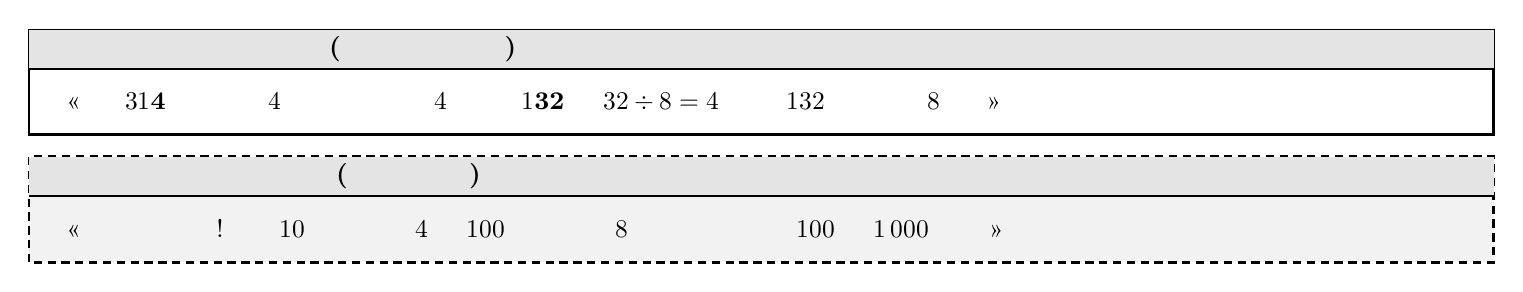
\begin{tikzpicture}[x=1cm, y=1cm, every node/.style={font=\fontsize{9.2pt}{13pt}\selectfont, text=black}]
  \draw[black, line width=0.95pt, fill=white] (0,1.62) rectangle (18.6,2.95);
  \fill[headband] (0,2.45) rectangle (18.6,2.95);
  \draw[black, line width=0.65pt] (0,2.45) -- (18.6,2.45);
  \node[anchor=west] at (0.28,2.70) {\textbf{ប្រអប់សន្ទនាទី ១ ៖ ការអះអាងរបស់សុខា (ចាំបាច់ត្រូវផ្ទៀងផ្ទាត់)}};
  \node[anchor=west] at (0.35,2.04) {«ចំនួន $31\mathbf{4}$ បញ្ចប់ដោយលេខ $4$ ដូច្នេះវាចែកដាច់នឹង $4$ ហើយចំនួន $1\mathbf{32}$ មាន $32\div 8 = 4$ ដូច្នេះ $132$ ក៏ចែកដាច់នឹង $8$ ដែរ ។»};

  \draw[black, line width=0.95pt, densely dashed, fill=panelgray] (0,0) rectangle (18.6,1.34);
  \fill[headband] (0,0.84) rectangle (18.6,1.34);
  \draw[black, line width=0.65pt] (0,0.84) -- (18.6,0.84);
  \node[anchor=west] at (0.28,1.09) {\textbf{ប្រអប់សន្ទនាទី ២ ៖ ការជំទាស់របស់ដារី (សួររកហេតុផលគោលដប់)}};
  \node[anchor=west] at (0.35,0.42) {«មិនទាន់ប្រាកដទេសុខា! ព្រោះ $10$ មិនចែកដាច់នឹង $4$ ហើយ $100$ មិនចែកដាច់នឹង $8$ ទេ ទើបយើងត្រូវពិនិត្យ $100$ និង $1\,000$ ជាមុន ។»};
\end{tikzpicture}\par\vspace{3pt}
\begin{wlist}
  \item \textbf{ការទស្សន៍ទាយដំបូងរបស់ក្រុមប្អូន៖} \quad \chkbox\ សុខាត្រឹមត្រូវ \qquad \chkbox\ ដារីត្រឹមត្រូវ
  \item \textbf{មូលហេតុបឋម (សរសេរ ១ ឃ្លាខ្លី)៖} \blank{11.5cm}
\end{wlist}

% -------------------- ផ្នែក ខ ស្ថានីយទី១ (E2 Explore: Divisibility by 4) --------------------
\secbox{ផ្នែក ខ \enbf{(E2 Explore)} ៖ ស្ថានីយទី១ \enbf{---} ពិសោធន៍កញ្ចប់ ១០០ រកក្បួនចែកដាច់នឹង \enbf{4} (ទំ.១៧)}{៥.៥ នាទី \en{---} ដៃគូ}

\begin{wlist}
  \item \textbf{ជំហានទី ១៖} សង្កេតដ្យាក្រាមបំបែកតម្លៃ $100$ និង $10$ ក្រោមតួចែក $4$ (រូបភាពខាងក្រោមរៀបពីលើចុះក្រោម) ។
  \item \textbf{ជំហានទី ២៖} បំពេញតារាងបំបែកកញ្ចប់ $100 + \text{ពីរខ្ទង់ចុង}$ សម្រាប់លេខឧទាហរណ៍ទំ.១៧ និងឧទាហរណ៍ផ្ទុយ ។
\end{wlist}
\vspace{4pt}
\begin{center}
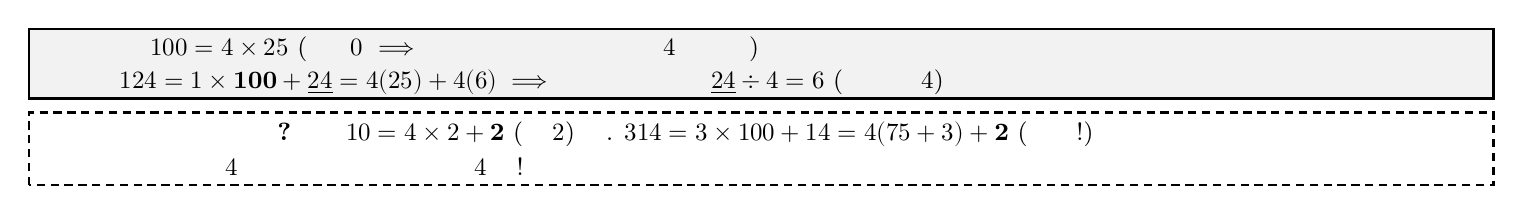
\begin{tikzpicture}[x=1cm, y=1cm, every node/.style={font=\fontsize{9.0pt}{12.8pt}\selectfont, text=black}]
  \draw[black, line width=0.95pt, fill=panelgray] (0,1.10) rectangle (18.6,1.98);
  \node[anchor=west] at (0.30,1.72) {\textbf{កញ្ចប់ ១០០៖} $100 = 4 \times 25$ (សំណល់ $0$ $\implies$ រាល់ចំនួនខ្ទង់រយឡើងលើ ចែកដាច់នឹង $4$ ជានិច្ច ។)};
  \node[anchor=west] at (0.30,1.30) {ឧទាហរណ៍ $124 = 1\times \mathbf{100} + \underline{24} = 4(25) + 4(6) \implies$ ពិនិត្យតែពីរខ្ទង់ចុង $\underline{24} \div 4 = 6$ (ចែកដាច់នឹង $4$) ។};

  \draw[black, line width=0.95pt, densely dashed, fill=white] (0,0) rectangle (18.6,0.92);
  \node[anchor=west] at (0.30,0.64) {\textbf{ហេតុអ្វីមើលតែ ១ ខ្ទង់ចុងមិនបាន?} ព្រោះ $10 = 4\times 2 + \mathbf{2}$ (សល់ $2$) ។ ឧ. $314 = 3\times 100 + 14 = 4(75+3)+\mathbf{2}$ (មិនដាច់!)};
  \node[anchor=west] at (0.30,0.23) {ដូច្នេះ លេខខាងចុងជាលេខ $4$ តែមួយខ្ទង់ \textbf{មិនធានា} ថាចែកដាច់នឹង $4$ ឡើយ!};
\end{tikzpicture}
\end{center}
\vspace{3pt}
{\renewcommand{\arraystretch}{1.52}
\fontsize{8.9pt}{12.5pt}\selectfont
\begin{tabular}{|C{1.85cm}|L{5.65cm}|C{2.35cm}|C{3.65cm}|C{3.45cm}|}
  \hline
  \cellcolor{panelgray}\textbf{ចំនួន} & \cellcolor{panelgray}\textbf{បំបែកជា ($\text{ខ្ទង់រយ} \times 100$) $+$ ២ ខ្ទង់ចុង} & \cellcolor{panelgray}\textbf{២ ខ្ទង់ចុង} & \cellcolor{panelgray}\textbf{ផលចែក ២ ខ្ទង់ចុងនឹង $4$} & \cellcolor{panelgray}\textbf{ចែកដាច់នឹង $4$ ឬទេ?} \\ \hline
  $124$ & $1\times 100 + 24$ & $24$ & $24 \div 4 = 6$ (សល់ $0$) & \chkbox\ ដាច់ \quad \chkbox\ ទេ \\ \hline
  $832$ & $8\times 100 + \blank{1.3cm}$ & \blank{1.2cm} & $32 \div 4 = \blank{1.4cm}$ & \chkbox\ ដាច់ \quad \chkbox\ ទេ \\ \hline
  $1\,000$ & $10\times 100 + \blank{1.3cm}$ & $00$ & $00 \div 4 = \blank{1.4cm}$ & \chkbox\ ដាច់ \quad \chkbox\ ទេ \\ \hline
  $2\,024$ & $20\times 100 + \blank{1.3cm}$ & \blank{1.2cm} & $24 \div 4 = \blank{1.4cm}$ & \chkbox\ ដាច់ \quad \chkbox\ ទេ \\ \hline
  $114$ & $1\times 100 + 14$ & \blank{1.2cm} & $14 \div 4 = 3$ (សល់ $\blank{0.6cm}$) & \chkbox\ ដាច់ \quad \chkbox\ ទេ \\ \hline
  $314$ & $\blank{1.0cm}\times 100 + \blank{1.3cm}$ & \blank{1.2cm} & $\blank{2.2cm}$ & \chkbox\ ដាច់ \quad \chkbox\ ទេ \\ \hline
\end{tabular}}
\vspace{5pt}
\begin{wlist}
  \item \textbf{សន្និដ្ឋានស្ថានីយទី១៖} ចំនួនមួយចែកដាច់នឹង $4$ កាលណា \blank{4.2cm} ចែកដាច់នឹង $4$ ព្រោះ $100 = 4 \times \blank{1.1cm}$ ។
  \item \textbf{សាកល្បងបង្កើតឧទាហរណ៍៖} សរសេរចំនួន ៣ ខ្ទង់ចុងលេខ $4$ ចំនួន ១ \textbf{ដាច់នឹង $4$}៖ \blank{1.45cm} និង ១ \textbf{មិនដាច់នឹង $4$}៖ \blank{1.45cm} ។
\end{wlist}


% ============================================================================
% ទំព័រទី ២ ៖ E2 ស្ថានីយទី២ (តួចែក 8) + E3 សំយោគ («ជាទូទៅ» 100% Verbatim + Venn + Warrant Bank)
% ============================================================================
\newpage

\secbox{ផ្នែក ខ (ត) \enbf{(E2 Explore)} ៖ ស្ថានីយទី២ \enbf{---} ពិសោធន៍ប្រអប់ ១\,០០០ រកក្បួនចែកដាច់នឹង \enbf{8} (ទំ.១៧)}{៥.៥ នាទី \en{---} ដៃគូ}

\begin{wlist}
  \item \textbf{ជំហានទី ១៖} ផ្ទៀងផ្ទាត់ថាតើ $100$ ចែកដាច់នឹង $8$ ដែរឬទេ រួចប្រៀបធៀបជាមួយ $1\,000 = 8 \times 125$ ។
  \item \textbf{ជំហានទី ២៖} បំពេញតារាងបំបែកប្រអប់ $1\,000 + \text{បីខ្ទង់ចុង}$ សម្រាប់ឧទាហរណ៍ ២ ទំ.១៧ និងឧទាហរណ៍ផ្ទុយ $132$ ។
\end{wlist}
\vspace{6pt}
\begin{center}
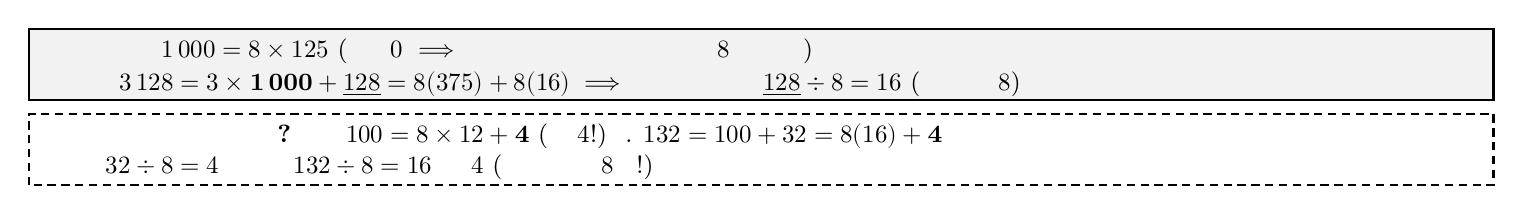
\begin{tikzpicture}[x=1cm, y=1cm, every node/.style={font=\fontsize{9.0pt}{12.8pt}\selectfont, text=black}]
  \draw[black, line width=0.95pt, fill=panelgray] (0,1.08) rectangle (18.6,1.98);
  \node[anchor=west] at (0.30,1.70) {\textbf{ប្រអប់ ១\,០០០៖} $1\,000 = 8 \times 125$ (សំណល់ $0$ $\implies$ រាល់ចំនួនខ្ទង់ពាន់ឡើងលើ ចែកដាច់នឹង $8$ ជានិច្ច ។)};
  \node[anchor=west] at (0.30,1.28) {ឧទាហរណ៍ $3\,128 = 3\times \mathbf{1\,000} + \underline{128} = 8(375) + 8(16) \implies$ ពិនិត្យបីខ្ទង់ចុង $\underline{128} \div 8 = 16$ (ចែកដាច់នឹង $8$) ។};

  \draw[black, line width=0.95pt, densely dashed, fill=white] (0,0) rectangle (18.6,0.90);
  \node[anchor=west] at (0.30,0.62) {\textbf{ហេតុអ្វីមើលតែ ២ ខ្ទង់ចុងមិនបាន?} ព្រោះ $100 = 8\times 12 + \mathbf{4}$ (សល់ $4$!) ឧ. $132 = 100 + 32 = 8(16) + \mathbf{4}$};
  \node[anchor=west] at (0.30,0.22) {ទោះជា $32 \div 8 = 4$ ក៏ដោយ តែ $132 \div 8 = 16$ \textbf{សល់ $4$} (មិនចែកដាច់នឹង $8$ ទេ!)};
\end{tikzpicture}
\end{center}
\vspace{5pt}
{\renewcommand{\arraystretch}{1.65}
\fontsize{8.9pt}{12.5pt}\selectfont
\begin{tabular}{|C{1.85cm}|L{5.45cm}|C{2.25cm}|C{3.95cm}|C{3.45cm}|}
  \hline
  \cellcolor{panelgray}\textbf{ចំនួន} & \cellcolor{panelgray}\textbf{បំបែកជា ($\text{ខ្ទង់ពាន់} \times 1\,000$) $+$ ៣ ខ្ទង់ចុង} & \cellcolor{panelgray}\textbf{៣ ខ្ទង់ចុង} & \cellcolor{panelgray}\textbf{ផលចែក ៣ ខ្ទង់ចុងនឹង $8$} & \cellcolor{panelgray}\textbf{ចែកដាច់នឹង $8$ ឬទេ?} \\ \hline
  $3\,128$ & $3\times 1\,000 + 128$ & $128$ & $128 \div 8 = 16$ (សល់ $0$) & \chkbox\ ដាច់ \quad \chkbox\ ទេ \\ \hline
  $5\,048$ & $5\times 1\,000 + \blank{1.3cm}$ & $048$ & $048 \div 8 = \blank{1.5cm}$ & \chkbox\ ដាច់ \quad \chkbox\ ទេ \\ \hline
  $7\,120$ & $7\times 1\,000 + \blank{1.3cm}$ & \blank{1.2cm} & $120 \div 8 = \blank{1.5cm}$ & \chkbox\ ដាច់ \quad \chkbox\ ទេ \\ \hline
  $4\,000$ & $4\times 1\,000 + \blank{1.3cm}$ & $000$ & $000 \div 8 = \blank{1.5cm}$ & \chkbox\ ដាច់ \quad \chkbox\ ទេ \\ \hline
  $132$ & $0\times 1\,000 + 132$ & $132$ & $132 \div 8 = 16$ (សល់ $\blank{0.6cm}$) & \chkbox\ ដាច់ \quad \chkbox\ ទេ \\ \hline
\end{tabular}}
\vspace{8pt}
\begin{wlist}
  \item \textbf{សន្និដ្ឋានស្ថានីយទី២៖} ចំនួនមួយចែកដាច់នឹង $8$ កាលណា \blank{4.2cm} ចែកដាច់នឹង $8$ ព្រោះ $1\,000 = 8 \times \blank{1.1cm}$ ។
  \item \textbf{ឧទាហរណ៍ផ្ទុយបង្កើតដោយសិស្ស៖} សរសេរចំនួន ៤ ខ្ទង់ ១ ដែល \textbf{ដាច់នឹង $4$ តែមិនដាច់នឹង $8$}៖ \blank{2.2cm}
  \item \textbf{ការពន្យល់មូលហេតុ៖} ២ ខ្ទង់ចុងគឺ \blank{1.6cm} (ចែកដាច់នឹង $4$) ប៉ុន្តែ ៣ ខ្ទង់ចុងគឺ \blank{1.8cm} (មិនចែកដាច់នឹង $8$) ។
\end{wlist}

\vspace{7pt}
% -------------------- ផ្នែក គ (E3 Explain — 100% Verbatim Textbook Box + Vertical Inclusion + Warrant Bank) --------------------
\secbox{ផ្នែក គ \enbf{(E3 Explain)} ៖ ប្រអប់ «ជាទូទៅ» ទំនាក់ទំនង \enbf{4} និង \enbf{8} ព្រមទាំងធនាគារហេតុផល}{៦ នាទី \en{---} សង្ខេបរួម}

\begin{tcolorbox}[
  enhanced, sharp corners, colback=panelgray, colframe=black, boxrule=1.0pt,
  left=8pt, right=8pt, top=9pt, bottom=9pt, boxsep=1pt
]
  {\muol\fontsize{9.8pt}{14pt}\selectfont ជាទូទៅ} \textbf{(សៀវភៅសិក្សាគោល ទំ.១៧ — ចងចាំ ១០០\%)៖}
  \begin{subwlist}
    \item មួយចំនួនចែកដាច់នឹង 4 កាលណាវាមានលេខខាងចុងពីរខ្ទង់ចែកដាច់នឹង 4
    \item មួយចំនួនចែកដាច់នឹង 8 កាលណាវាមានលេខខាងចុងបីខ្ទង់ចែកដាច់នឹង 8 ។
  \end{subwlist}
\end{tcolorbox}

\vspace{10pt}
\begin{center}
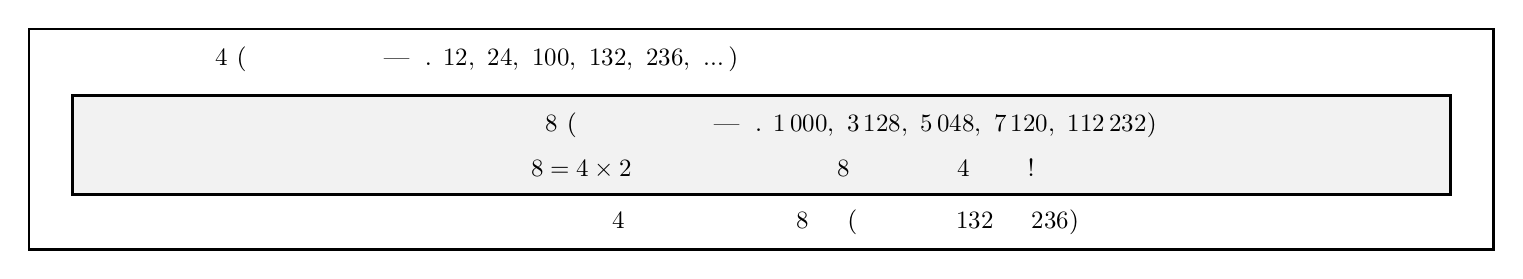
\begin{tikzpicture}[x=1cm, y=1cm, every node/.style={font=\fontsize{9.0pt}{12.5pt}\selectfont, text=black}]
  \draw[black, line width=0.95pt, fill=white] (0,0) rectangle (18.6,2.80);
  \node[anchor=west] at (0.35,2.42) {\textbf{សំណុំចំនួនចែកដាច់នឹង $4$} (ពិនិត្យ ២ ខ្ទង់ចុង — ឧ. $12,\ 24,\ 100,\ 132,\ 236,\ \dots$)};

  \draw[black, line width=1.05pt, fill=panelgray] (0.55,0.70) rectangle (18.05,1.95);
  \node at (9.30,1.58) {\textbf{សំណុំរង៖ ចំនួនចែកដាច់នឹង $8$} (ពិនិត្យ ៣ ខ្ទង់ចុង — ឧ. $1\,000,\ 3\,128,\ 5\,048,\ 7\,120,\ 112\,232$)};
  \node at (9.30,1.04) {ព្រោះ $8 = 4\times 2$ ដូច្នេះគ្រប់ចំនួនចែកដាច់នឹង $8$ តែងចែកដាច់នឹង $4$ ជានិច្ច!};

  \node at (9.30,0.34) {\textbf{ប្រយ័ត្ន៖} ចំនួនចែកដាច់នឹង $4$ \textbf{មិនប្រាកដ} ថាចែកដាច់នឹង $8$ ឡើយ (ឧទាហរណ៍ផ្ទុយ៖ $132$ និង $236$) ។};
\end{tikzpicture}
\end{center}

\vspace{10pt}
\begin{tcolorbox}[
  enhanced, sharp corners, colback=white, colframe=black, boxrule=0.9pt,
  left=8pt, right=8pt, top=9pt, bottom=9pt, boxsep=1pt
]
  {\muol\fontsize{9.5pt}{13.5pt}\selectfont ធនាគារហេតុផល \enbf{(Warrant Bank)} សម្រាប់សរសេរយោងក្នុងលំហាត់៖}
  \begin{wlist}
    \item[\cnum{1}] \textbf{ដាច់នឹង $4$៖} លេខខាងចុងពីរខ្ទង់ចែកដាច់នឹង $4$ (រួមទាំង $00,\ 04,\ 08$) ។
    \item[\cnum{2}] \textbf{ដាច់នឹង $8$៖} លេខខាងចុងបីខ្ទង់ចែកដាច់នឹង $8$ (រួមទាំង $000,\ 008,\ 048$) ។
    \item[\cnum{3}] \textbf{វិបាក $8 \implies 4$៖} ចែកដាច់នឹង $8 \implies$ ចែកដាច់នឹង $4$ ជានិច្ច (តែច្រាសមកវិញមិនពិត ឧ. $132$) ។
    \item[\cnum{4}] \textbf{លក្ខខណ្ឌរួមគ្នា៖} ដើម្បីឱ្យចែកដាច់នឹង $4$ ផង និង $8$ ផង ត្រូវរកលេខបំពេញលក្ខខណ្ឌ \cnum{1} រួចផ្ទៀងលក្ខខណ្ឌ \cnum{2} ។
  \end{wlist}
\end{tcolorbox}


% ============================================================================
% ទំព័រទី ៣ ៖ E4 លំហាត់គំរូ (EFWE + EIA) + E5 ប្រតិបត្តិ + វិនិច្ឆ័យ A–D + សំបុត្រចេញ + កិច្ចការផ្ទះ
% ============================================================================
\newpage

\secbox{ផ្នែក ឃ \enbf{(E4 Elaborate)} ៖ លំហាត់គំរូ ទំ.១៧ និងសំណួរត្រិះរិះ \enbf{EIA}}{១០ នាទី \en{---} សម្រាយផ្លូវការ}

\begin{tcolorbox}[
  enhanced, sharp corners, colback=white, colframe=black, boxrule=0.9pt,
  left=8pt, right=8pt, top=4pt, bottom=4.5pt, boxsep=1pt
]
  {\muol\fontsize{9.3pt}{13.5pt}\selectfont លំហាត់គំរូ ១ \enbf{(}ទំ.១៧\enbf{)} ៖} \textbf{គេឱ្យចំនួន $6$ ខ្ទង់ $112\,23\,\numbox\,$ ។ ចូរបំពេញលេខក្នុងប្រអប់ដើម្បីឱ្យចែកដាច់នឹង $4$ ផង និង $8$ ផង ។}\\[2pt]
  $\displaystyle\begin{aligned}
    &\text{ជំហាន ១ (ពិនិត្យលក្ខខណ្ឌ } 4 \text{ តាមកូដ \cnum{1})៖} &&3\square \div 4 \implies \square \in \{2,\ 6\} \quad (\text{ព្រោះ } 32 = 4\times 8 \text{ និង } 36 = 4\times 9) \\
    &\text{ជំហាន ២ (ពិនិត្យលក្ខខណ្ឌ } 8 \text{ តាមកូដ \cnum{2})៖} &&\text{ករណី } \square = 2 \text{៖ } 232 \div 8 = \blank{1.1cm} \text{ (សំណល់ } \blank{0.6cm} \implies \text{យក / មិនយក?)} \\
    &&&\text{ករណី } \square = 6 \text{៖ } 236 \div 8 = 29 \text{ (សំណល់ } \blank{0.6cm} \implies \text{មិនចែកដាច់នឹង } 8\text{!)} \\
    &\text{សន្និដ្ឋាន៖} &&\text{ដូច្នេះ } \square = \blank{0.9cm} \text{ ហើយចំនួននោះគឺ } \blank{2.2cm} \text{ ។}
  \end{aligned}$\\[3pt]
  \colorbox{panelgray}{\parbox{17.8cm}{\textbf{សំណួរ \en{EIA Looking-Back} (១ នាទី)៖} ហេតុអ្វីគេមិនយក $\square = 6$ ($112\,236$) បើទោះជា $36$ ចែកដាច់នឹង $4$? ចម្លើយ៖ \blank{3.6cm}}}
\end{tcolorbox}

\vspace{4pt}
\begin{tcolorbox}[
  enhanced, sharp corners, colback=white, colframe=black, boxrule=0.9pt,
  left=8pt, right=8pt, top=4pt, bottom=4.5pt, boxsep=1pt
]
  {\muol\fontsize{9.3pt}{13.5pt}\selectfont លំហាត់គំរូ ២ \enbf{(}ទំ.១៧\enbf{)} ៖} \textbf{ពីឆ្នាំ $1999$ ដល់ឆ្នាំ $2010$ តើឆ្នាំណាខ្លះចែកដាច់នឹង $4$ ផង និង $8$ ផង?}\\[2pt]
  $\displaystyle\begin{aligned}
    &\text{ជំហាន ១ (ឆ្នាំគូចែកដាច់នឹង } 4 \text{ តាម \cnum{1})៖} &&2000 \to 00 \div 4 = 0\text{ (យក)};\;\; 2004 \to 04 \div 4 = \blank{0.7cm};\;\; 2008 \to 08 \div 4 = \blank{0.7cm} \\
    &\text{ជំហាន ២ (ពិនិត្យ ៣ ខ្ទង់ចុងនឹង } 8 \text{ តាម \cnum{2})៖} &&2000 \to 000 \div 8 = \blank{0.8cm};\quad 2004 \to 004 \div 8 = \text{សល់ } \blank{0.6cm} \\
    &&&2008 \to 008 \div 8 = \blank{0.8cm} \\
    &\text{សន្និដ្ឋាន៖} &&\text{ចម្លើយចន្លោះ $2001$--$2010$ តាមសៀវភៅគោលគឺ } \blank{1.4cm} \\
    &&&\text{(ប្រសិនបើរាប់ចាប់ពីឆ្នាំ $2000$ មាន៖ } \blank{2.6cm} \text{) ។}
  \end{aligned}$
\end{tcolorbox}

% -------------------- ផ្នែក ង (E5 Evaluate: ប្រតិបត្តិ 734□0 + បិទ E1 + វិនិច្ឆ័យ A–D + សំបុត្រចេញ + កិច្ចការផ្ទះ) --------------------
\secbox{ផ្នែក ង \enbf{(E5 Evaluate)} ៖ ប្រតិបត្តិទំ.១៧ វិនិច្ឆ័យ \enbf{A--D} សំបុត្រចេញ និងកិច្ចការផ្ទះ}{១០ នាទី \en{+} ផ្ទះ $\le$២ នាទី}

\begin{wlist}
  \item \textbf{១. ប្រតិបត្តិទំ.១៧ (ជាក្រុម ៣ នាក់ — ៤ នាទី)៖} គេមានចំនួនប្រាំខ្ទង់ $734\,\numbox\,0$ ។ បំពេញលេខក្នុងប្រអប់ដើម្បីឱ្យចែកដាច់៖
\end{wlist}
$\displaystyle\begin{aligned}
  &\text{ក. ចែកដាច់នឹង } 4 \text{ (មើល } \square 0 \div 4\text{)៖} &&00,\ 20,\ 40,\ 60,\ 80 \implies \square \in \{\blank{3.6cm}\} \quad (\text{កុំភ្លេចលេខ } 0\text{!}) \\
  &\text{ខ. ចែកដាច់នឹង } 8 \text{ (មើល } 4\square 0 = 400 + \square 0\text{)៖} &&400 \div 8 = 50;\quad 440 \div 8 = \blank{0.9cm};\quad 480 \div 8 = \blank{0.9cm} \\
  &&&\implies \square \in \{\blank{2.8cm}\} \\
  &\text{គ. បិទបេសកកម្ម \en{E1} (សុខា vs ដារី)៖} &&\chkbox\ \text{ដារីត្រូវ ព្រោះ } 314\ (14\div 4 \text{ សល់ } \blank{0.6cm}) \\
  &&&\text{និង } 132\ (132\div 8 = 16 \text{ សល់ } \blank{0.6cm}) \text{ មិនចែកដាច់! }
\end{aligned}$

\vspace{4pt}
\noindent\textbf{២. វិនិច្ឆ័យរហ័ស \en{A--D} (៣ នាទី)៖} គូស \ding{51} លើ \textbf{ត្រូវ} ឬ \textbf{ខុស} រួចសរសេរលេខកូដហេតុផល \cnum{1}--\cnum{4} ហើយលើកម្រាមដៃបង្ហាញគ្រូ (១=ត្រូវ, ២=ខុស)៖\\[3pt]
{\renewcommand{\arraystretch}{1.35}
\fontsize{8.8pt}{12.2pt}\selectfont
\begin{tabular}{|C{0.75cm}|L{10.1cm}|C{2.45cm}|L{4.05cm}|}
  \hline
  \cellcolor{panelgray}\textbf{ល.រ} & \cellcolor{panelgray}\textbf{អំណះអំណាងដែលត្រូវពិនិត្យ} & \cellcolor{panelgray}\textbf{វិនិច្ឆ័យ} & \cellcolor{panelgray}\textbf{កូដយោង \cnum{1}--\cnum{4} / ហេតុផល} \\ \hline
  \textbf{A} & «$314$ បញ្ចប់ដោយលេខ $4$ ដូច្នេះ $314$ ចែកដាច់នឹង $4$ ។» & \chkbox\ ត្រូវ \ \chkbox\ ខុស & កូដ \blank{0.6cm}៖ \blank{2.5cm} \\ \hline
  \textbf{B} & «$132$ មាន ២ ខ្ទង់ចុង $32$ ចែកដាច់នឹង $8$ ដូច្នេះ $132$ ចែកដាច់នឹង $8$ ។» & \chkbox\ ត្រូវ \ \chkbox\ ខុស & កូដ \blank{0.6cm}៖ \blank{2.5cm} \\ \hline
  \textbf{C} & «ប្រសិនបើចំនួនមួយចែកដាច់នឹង $8$ នោះវាច្បាស់ជាចែកដាច់នឹង $4$ ជានិច្ច ។» & \chkbox\ ត្រូវ \ \chkbox\ ខុស & កូដ \blank{0.6cm}៖ \blank{2.5cm} \\ \hline
  \textbf{D} & «ក្នុង $734\square 0$ អាចដាក់ $\square = 0$ ដើម្បីឱ្យ $73\,400$ ចែកដាច់នឹង $4$ និង $8$ បាន ។» & \chkbox\ ត្រូវ \ \chkbox\ ខុស & កូដ \blank{0.6cm}៖ \blank{2.5cm} \\ \hline
\end{tabular}}

\vspace{4pt}
\begin{tcolorbox}[
  enhanced, sharp corners, colback=panelgray, colframe=black, boxrule=0.95pt,
  left=8pt, right=8pt, top=4pt, bottom=4pt, boxsep=1pt
]
  {\muol\fontsize{9.2pt}{13pt}\selectfont ៣. សំបុត្រចេញ ៩០ វិនាទី \enbf{(Exit Ticket --- }ធ្វើដោយឯករាជ្យ\enbf{)}៖} រកលេខ ១ ខ្ទង់ក្នុង $5\,27\,\numbox\,$ ឱ្យចែកដាច់នឹង $4$ ផង និង $8$ ផង៖\\[2pt]
  $\displaystyle\begin{aligned}
    &\text{ជំហាន ១ (ពិនិត្យ } 7\square \div 4\text{)៖ } \square \in \{\blank{1.6cm}\} \qquad
    &\text{ជំហាន ២ (ពិនិត្យ } 27\square \div 8\text{)៖ } \square = \blank{1.1cm} \implies \text{ចំនួនគឺ } 5\,27\blank{0.7cm} \text{ ។}
  \end{aligned}$
\end{tcolorbox}

\vspace{4pt}
\begin{tcolorbox}[
  enhanced, sharp corners, colback=white, colframe=black, boxrule=0.95pt,
  left=8pt, right=8pt, top=4pt, bottom=4pt, boxsep=1pt
]
  {\muol\fontsize{9.2pt}{13pt}\selectfont ៤. កិច្ចការផ្ទះ និងបណ្ដាំផ្ញើត្រៀមម៉ោងក្រោយ}
  \begin{wlist}
    \item \textbf{លំហាត់ ១៖} កំណត់ថាតើចំនួន $4\,216;\ 9\,132;\ 12\,500;\ 8\,408$ ចែកដាច់នឹង $4$ ឬ $8$ ឬទាំងពីរ ដោយបង្ហាញ ២ ខ្ទង់ និង ៣ ខ្ទង់ចុង ។
    \item \textbf{លំហាត់ ២៖} បំពេញលេខក្នុងប្រអប់នៃ $61\,3\square 6$ ដើម្បីឱ្យចែកដាច់នឹង $4$ ផង និង $8$ ផង (ប្រយ័ត្នអាចមានច្រើនជាង ១ ចម្លើយ) ។
    \item \textbf{បណ្ដាំផ្ញើ៖} អានមុន \textbf{១.២ លក្ខណៈចែកដាច់នៃផលបូកនិងផលដក (សៀវភៅសិក្សាគោល ទំ.១៨)} ។
  \end{wlist}
\end{tcolorbox}

\end{document}
